%%%%%%%%%%%%%%%%%%%%%%%%%%%%%%%%%%%%%%%%%%%%%%%%%%%%%%%%%%%%%%%%%%%%%%%%%%%%%
%% Original default rstudio/pandoc latex file
%% upated by @jhollist 09/15/2014
%% inspired by @cboetting https://github.com/cboettig/template and
%% @rmflight blog posts:
%% http://rmflight.github.io/posts/2014/07/analyses_as_packages.html 
%% http://rmflight.github.io/posts/2014/07/vignetteAnalysis.html).  
%%%%%%%%%%%%%%%%%%%%%%%%%%%%%%%%%%%%%%%%%%%%%%%%%%%%%%%%%%%%%%%%%%%%%%%%%%%%%

\documentclass[11pt,a4paper]{article}
\usepackage[T1]{fontenc}
\usepackage{lmodern}
\usepackage{amssymb,amsmath}
\usepackage{ifxetex,ifluatex}
\usepackage{fixltx2e} % provides \textsubscript
% use upquote if available, for straight quotes in verbatim environments
\IfFileExists{upquote.sty}{\usepackage{upquote}}{}
\ifnum 0\ifxetex 1\fi\ifluatex 1\fi=0 % if pdftex
  \usepackage[utf8]{inputenc}
\else % if luatex or xelatex
  \ifxetex
    \usepackage{mathspec}
    \usepackage{xltxtra,xunicode}
  \else
    \usepackage{fontspec}
  \fi
  \defaultfontfeatures{Mapping=tex-text,Scale=MatchLowercase}
  \newcommand{\euro}{€}
\fi
% use microtype if available
\IfFileExists{microtype.sty}{\usepackage{microtype}}{}
\usepackage{color}
\usepackage{fancyvrb}
\newcommand{\VerbBar}{|}
\newcommand{\VERB}{\Verb[commandchars=\\\{\}]}
\DefineVerbatimEnvironment{Highlighting}{Verbatim}{commandchars=\\\{\}}
% Add ',fontsize=\small' for more characters per line
\usepackage{framed}
\definecolor{shadecolor}{RGB}{248,248,248}
\newenvironment{Shaded}{\begin{snugshade}}{\end{snugshade}}
\newcommand{\KeywordTok}[1]{\textcolor[rgb]{0.13,0.29,0.53}{\textbf{{#1}}}}
\newcommand{\DataTypeTok}[1]{\textcolor[rgb]{0.13,0.29,0.53}{{#1}}}
\newcommand{\DecValTok}[1]{\textcolor[rgb]{0.00,0.00,0.81}{{#1}}}
\newcommand{\BaseNTok}[1]{\textcolor[rgb]{0.00,0.00,0.81}{{#1}}}
\newcommand{\FloatTok}[1]{\textcolor[rgb]{0.00,0.00,0.81}{{#1}}}
\newcommand{\CharTok}[1]{\textcolor[rgb]{0.31,0.60,0.02}{{#1}}}
\newcommand{\StringTok}[1]{\textcolor[rgb]{0.31,0.60,0.02}{{#1}}}
\newcommand{\CommentTok}[1]{\textcolor[rgb]{0.56,0.35,0.01}{\textit{{#1}}}}
\newcommand{\OtherTok}[1]{\textcolor[rgb]{0.56,0.35,0.01}{{#1}}}
\newcommand{\AlertTok}[1]{\textcolor[rgb]{0.94,0.16,0.16}{{#1}}}
\newcommand{\FunctionTok}[1]{\textcolor[rgb]{0.00,0.00,0.00}{{#1}}}
\newcommand{\RegionMarkerTok}[1]{{#1}}
\newcommand{\ErrorTok}[1]{\textbf{{#1}}}
\newcommand{\NormalTok}[1]{{#1}}
\usepackage{graphicx}
% Redefine \includegraphics so that, unless explicit options are
% given, the image width will not exceed the width of the page.
% Images get their normal width if they fit onto the page, but
% are scaled down if they would overflow the margins.
\makeatletter
\def\ScaleIfNeeded{%
  \ifdim\Gin@nat@width>\linewidth
    \linewidth
  \else
    \Gin@nat@width
  \fi
}
\makeatother
\let\Oldincludegraphics\includegraphics
{%
 \catcode`\@=11\relax%
 \gdef\includegraphics{\@ifnextchar[{\Oldincludegraphics}{\Oldincludegraphics[width=\ScaleIfNeeded]}}%
}%
\ifxetex
  \usepackage[setpagesize=false, % page size defined by xetex
              unicode=false, % unicode breaks when used with xetex
              xetex]{hyperref}
\else
  \usepackage[unicode=true]{hyperref}
\fi
\hypersetup{breaklinks=true,
            bookmarks=true,
            pdfauthor={},
            pdftitle={Data management procedures for reproducible research pipelines},
            colorlinks=true,
            citecolor=blue,
            urlcolor=blue,
            linkcolor=magenta,
            pdfborder={0 0 0}}
\urlstyle{same}  % don't use monospace font for urls
\setlength{\parindent}{0pt}
\setlength{\parskip}{6pt plus 2pt minus 1pt}
\setlength{\emergencystretch}{3em}  % prevent overfull lines
\setcounter{secnumdepth}{5}

%%%%%%%%%%%%%%%%%%%%%%%%%%%%%%%%%%%%%%%%%%%%%%%%%%%%%%%%
%Changes borrowed from @cboettig, added by @jhollist 
% A modified page layout 
\textwidth 6.75in
\oddsidemargin -0.15in
\evensidemargin -0.15in
\textheight 9in
\topmargin -0.5in
\usepackage{lineno} % add 
%%%%%%%%%%%%%%%%%%%%%%%%%%%%%%%%%%%%%%%%%%%%%%%%%%%%%%%%

%%%%%%%%%%%%%%%%%%%%%%%%%%%%%%%%%%%%%%%%%%%%%%%%%%%%%%%%
%%Packages and layout changes by @jhollist 09/15/2014
\usepackage{ragged2e}
\usepackage[font=normalsize]{caption}
  \usepackage[singlespacing]{setspace}
\usepackage{parskip}
\usepackage{fancyhdr}
\pagestyle{fancy}
\fancyhf{}
\renewcommand{\headrulewidth}{0pt}
%\rfoot{\today}
\cfoot{\thepage}
%%Changed default abstract width and added lines
\renewenvironment{abstract}{
  \hfill\begin{minipage}{1\textwidth}
  \rule{\textwidth}{1pt}\vspace{5pt}
  \normalsize
  \begin{justify}
  \bfseries\abstractname\vspace{5pt}
  \end{justify}}
  {\par\noindent\rule{\textwidth}{1pt}\end{minipage}
}
%%%%%%%%%%%%%%%%%%%%%%%%%%%%%%%%%%%%%%%%%%%%%%%%%%%%%%%%

\title{Data management procedures for reproducible research pipelines}
\author{
}
\date{}
\usepackage{graphicx}
\usepackage{url}
\usepackage{hyperref}
\usepackage{tikz}
\usetikzlibrary{calc}

\begin{document}
%%Edited by @jhollist 09/15/2014
%%Adds title from YAML
\begin{singlespace}
\begin{center}
\huge Data management procedures for reproducible research pipelines
\end{center}
%%Adds Author, correspond email asterisk, and affilnum from YAML
\begin{center}
\large
\end{center}
%%Adds affiliations from YAML
\begin{justify}
\footnotesize \emph{ 
}
%%Adds corresponding author email(s) from YAML
\newcounter{num}
\setcounter{num}{1}
\\[0.1cm]
\footnotesize \emph{ 
}
\end{justify}
%%Adds date from YAML
\normalsize

\begin{abstract}
This unpublished working paper was written to accompany the material
included in the PhD thesis `Using Reproducible Research Pipelines to
Help Disentangle Health Effects of Environmental Changes from Social
Factors' by Ivan Hanigan (2016). It sets out the key data management and
analysis principles that were found to be most effective for the
reproducibile synthesis and integration of heterogeneous datasets for
analysis and reporting. The draft was last updated \today. The version
submitted with the thesis is available as part of a Github repository at
\href{https://github.com/swish-climate-impact-assessment/swish_data_management_procedures/blob/master/swish-dmp-report.pdf}{\url{https://github.com/swish-climate-impact-assessment/swish_data_management_procedures/blob/master/swish-dmp-report.pdf}}.
\end{abstract}
\end{singlespace}

{
\hypersetup{linkcolor=black}
\setcounter{tocdepth}{2}
\tableofcontents
}

\clearpage
\doublespace

\section{Introduction}\label{introduction}

There is a need for developing an evidence based set of best practice
guidelines for data management procedures in implementing reproducible
research pipelines in epidemiology (Peng 2015). The examples drawn
together in this report come from experiences and use-cases found in an
eco-social epidemiologic research context. The emerging paradigm of
eco-social epidemiology is inherently concerned with complex systems and
integrating heterogenous data sources to aid recognition of patterns in
the environmental and social determinants of population health
(McMichael 2013). This document outlines a suite of data management
procedures that have been found to effectively assist the development of
reproducible research pipelines.

\section{Configuration versus convention: The case for standardised
approaches}\label{configuration-versus-convention-the-case-for-standardised-approaches}

Reproducibility is the ability to recompute the results of a data
analysis with the original data. It is possible to have analyses that
are reproducible with varying degrees of difficulty. A data analysis
might be reproducible but require thousands of hours of work. A primary
challenge for reproducible data analysis is to make analyses that are
\emph{easy} to reproduce.

In essence this requires attention to be turned to the issue of how the
data and analytical steps amassed -- toward a reality where this is
archived and there is a good understanding all round as to how the study
were set up and conducted. Different assumptions or different treatment
of the data could conceivably lead to different inferences and
conclusions being drawn, such as in the example shown by Silberzahn \&
Uhlmann (2015) in which 29 research teams were given the same dataset
but reached a wide variety of conclusions using different methods on the
same dataset to answer the same question.

This is partly because of an underlying complexity in the information
drawn from complex systems involving multi-causality, and partly because
of different assumptions and different backgrounds and viewpoints. A
finding that a variable does or does not cause a disease, might be drawn
honestly from the same set of data.

The techniques of pipelines described here are targeting the integrity
of the process of data selection, the robustness and suitableness of the
methods used, a commonsense and well-argued selection of health outcomes
and environmental or social exposures, and the clarity and transparency
of the methods used.

To achieve this, a guiding principle is that analysts should effectively
implement `pipelines' of method steps and tools. Standardised and
evidence-based methods based on conventions developed from many data
analysts approaching the problems in a similar way should be used,
rather than each analyst configuring a pipeline to suit particular
individual or domain-specific preferences (Borer \emph{et al.} 2009;
White \emph{et al.} 2013).

Noble (2009) points out that `the principles behind organizing and
documenting computational experiments are often learned on the fly, and
this learning is strongly influenced by personal predilections'. Leek \&
Peng (2015) describe this as data analysis being `taught through an
apprenticeship model, and different disciplines develop their own
analysis subcultures'. By codifying what an appropriate pipeline would
contain, data analysis will be more robust. According to Peng (2015),
there should not be a `lonely data analyst' coming up with their own
method. If a researcher conducted an analysis using an evidence-based
reproducible research pipeline `you could at least have a sense that
something reasonable was done' and be confident that you could easily
check what had been done if you needed to.

\subsection{The core components of a
pipeline}\label{the-core-components-of-a-pipeline}

Peng et al. (2006) distilled a core set of components for
reproducibility from earlier work including that of Schwab et al.
(2000). These are:

\begin{itemize}
\itemsep1pt\parskip0pt\parsep0pt
\item
  Hypothesis and design
\item
  Data (measurement, pre-processing, analytic)
\item
  Analysis Methods
\item
  Documentation (of all steps)
\item
  Distribution (of the paper, data and code).
\end{itemize}

\subsection{Hypothesis and design}\label{hypothesis-and-design}

The first stage of the pipeline is hypothesis generation and study
design. In this stage documentation should explain the literature base
supporting the study, the decisions made in selection of explanatory
factors for inclusion, decisions made such as the experimental unit,
observational unit, measurement method, as well as spatial or temporal
extent. This information will also be needed for ethical review and
approval.

\subsection{Data}\label{data}

The data that were measured should be well managed, however the
requirements for accessing the original raw data are less important than
for the analytical dataset. Descriptions of how the measured data were
transformed into the analytic data should be available. Public data
repositories or institutional services such as university libraries
should be used to ensure longevity of the data storage.

\subsection{Methods}\label{methods}

The software code underlying the principal results needs to be made
available. In addition, the computer environment necessary to execute
that code should be described adequately to `deploy' a new computer
set-up that can reproduce the computations needed.

\subsection{Documentation}\label{documentation}

Adequate documentation of the code and data should be available to
enable others to repeat the analyses and to conduct other similar ones.
This can take the form of metadata, reports, journal papers or even
books (Peng \& Dominici 2008). Indeed textbooks on statistical methods
can benefit greatly from being accompanied by data and analytical code
to enhance their pedagogic functions (Barnett \& Dobson 2010; Barnett
\emph{et al.} 2014).

An important underpinning to reproducible research is the reproducible
report. This is the ultimate form of documentation because the
information that represents the outputs of the research is written
alongside the code that performs the computations that are being
described. There has been many recent advances made in terms of tools
for reproducible reports such as R markdown and knitr (Xie 2014).

Metadata should be created and maintained as a priority task at all
stages of the data analysis process. An international standard should be
preferred over selectively choosing what information one collects and
what fieldnames one uses to describe each item of documentation.
Ecological Metadata Language (EML) and the Data Documentation
Inititative (DDI) are two such standards that offer useful semantic
constructs for describing epidemiological data.

\subsection{Distribution}\label{distribution}

Distribution or dissemination of the material needs to use a standard
method if they are to be used by others. It is not enough just to
provide access to the software and data, but also adequate documentation
is required to explain and potentially assist downstream users to piece
these together.

\section{Procedures when conducting a reproducible research
analysis}\label{procedures-when-conducting-a-reproducible-research-analysis}

Having defined above the principle components for a pipeline there are
procedural questions about how to go about compiling those. The key
steps include:

\begin{itemize}
\itemsep1pt\parskip0pt\parsep0pt
\item
  Data Management Plans and Data Inventories
\item
  Tracking method steps
\item
  Developing code
\item
  Maintaining data storage
\item
  Writing reports
\item
  Distributing the materials.
\end{itemize}

\subsection{Data management plan and data
inventory}\label{data-management-plan-and-data-inventory}

In eco-social epidemiology there is a need for a data management plan
and a data inventory that enables individual scientists, or
multidisciplinary teams of scientists, to manage large and heterogeneous
collections of disparate data sources efficiently. Keeping track of all
the elements of a linked health, social and environmental database is
very challenging, despite major improvements in data management
software, web-portals and virtual laboratories (Fleming \emph{et al.}
2014).

Effective data management policies and procedures are essential in
managing data-related risk. Such risks include data loss or corruption,
technological obsolescence, breaches of privacy or copyright, and errors
or misuse. Misuse may be due either to unintended user misunderstandings
about data attributes (no dataset is perfect and self-explanatory, see
Michener et al. (1997)) or intentional mis-use for malicious or selfish
reasons (for example the misuse of data by Bjorn Lomborg to support the
argument that environmental health conditions are actually improving.
See Bodnar et al. (2004) for a discussion on Lomborg's misuse of data.
There have also been notable examples of mistakes in data analyses used
for climate change science. See Cai et al. (2010) for a discussion of
one such case. The careful storage and curation of datasets is also
critical because data from many studies are lost (Pullin \& Salafsky
2010; Vines \emph{et al.} 2014).

Data management plans are needed for developing procedures and processes
to keep data safe. There is an issue when ensuring that all relevant
data are collected in deciding what is relevant. Keeping an up-to-date
data inventory and careful organisation of all folders and files helps
mitigate these problems.

Whether data management is the responsibility of the individuals
collecting or collating it, or of the lead scientist, clarity on how and
where data are stored and who manages it is vital, as is a `succession
plan' that sets out the vision of the data collections preservation and
re-use into the future.

\subsection{Case study 1: Ecological Metadata Language (EML) and folder
structure}\label{case-study-1-ecological-metadata-language-eml-and-folder-structure}

For data to be reused in the future, metadata and documentation need to
be carefully prepared to allow future users (including the original
collector) to find and understand the data (Michener et al. 1997).
Metadata should be associated with the data and adhere to a standard
schema. This example shows the use of the Ecological Metadata Language
(EML).

Good metadata requires sufficient detail to describe the collection
process and to record decisions that were made during the design phase
about the use of different sampling methods. Time and effort may be
saved by considering metadata requirements at the commencement of a
study, rather than trying to recall all the details later. If metadata
adheres to a standard schema, it can be used in catalogues to enable
fast searching and retrieval, or in machine-to-machine data queries that
assist data access and use.

In EML the elements of any dataset can be seen as a nested hierarchy at
three levels:

\begin{enumerate}
\def\labelenumi{\arabic{enumi}.}
\itemsep1pt\parskip0pt\parsep0pt
\item
  The Project level: this is an overarching grouping of data. It might
  be indicative of the principal investigator or organisation who
  provided the data, or a programme of research studies (sub-projects).
\item
  The Dataset level: this is a distinct grouping of data that might be
  organised around a particular time period or geographical region.
\item
  The Entity level: This grouping of data includes data files (such as
  tables in CSV or Excel, shapefiles and raster images) or documents
  (such as metadata descriptions or related publications).
\end{enumerate}

This conceptual framework can be very useful for the organisation of the
work constituting a single pipeline, as well as when working with
multiple pipelines within several projects.

\begin{figure}[htbp]
\centering
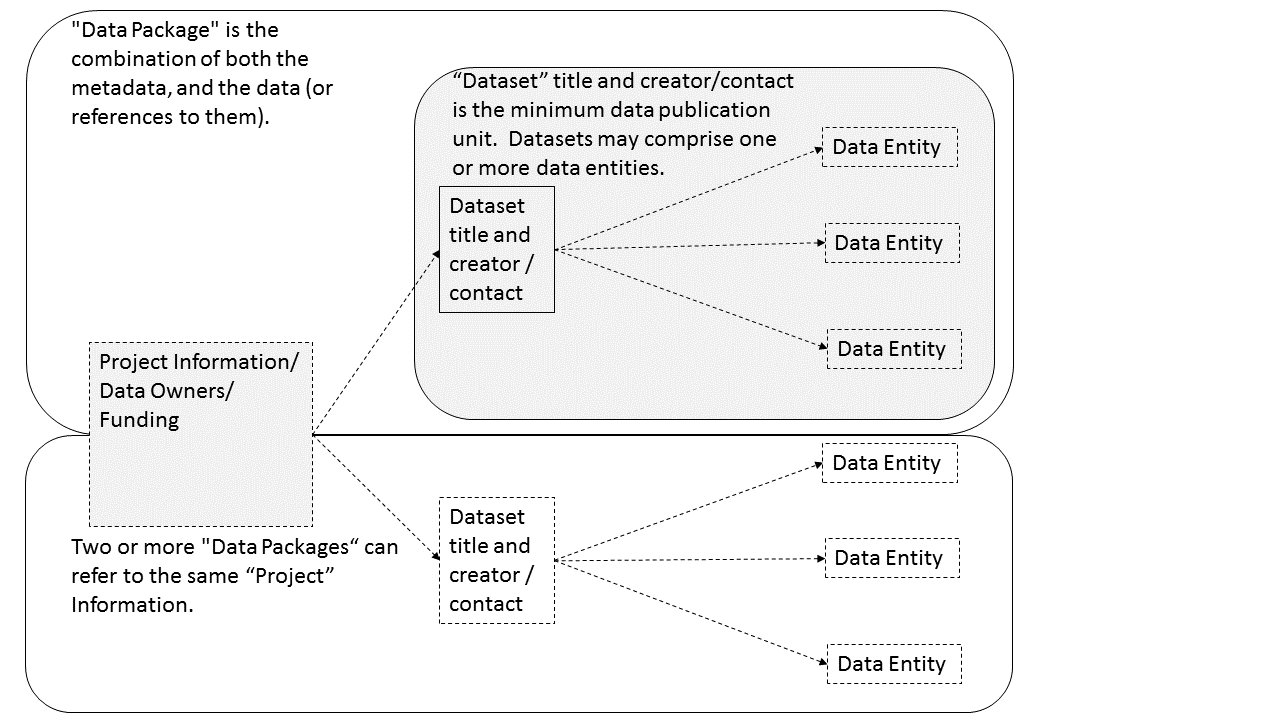
\includegraphics{images/EML_project.png}
\caption{images/EML\_project.png}
\end{figure}

\subsection{Data storage and access}\label{data-storage-and-access}

Some datasets such as sensitive personal information about suicide or
climate change scenarios with restrictions due to privacy and
confidentiality rules, or because of protected intellectual property,
need to be accessed in a restricted way. This complicates the
implementation of the method of pipelines which dictates that all the
steps, models and assumptions need to be made transparent and available
for scientific debate even though the datasets may require authorisation
to access. Restrictions around access to data have increased recently in
Australia. As an example the custodians of the national mortality
database made it virtually impossible to access these data for several
years after the discovery of an incident in which Australian population
health researcher Dr Stephen Begg was reported to have hacked into the
database in an illegal act (O'Keefe 2007). The subsequent investigation
by the data custodians led to a wide ranging modification to the
procedures for approval and provision of these data that make the access
much more restricted. Appropriate access to data is therefore required
to address this issue. In the work reported in the conference
presentation in this thesis, a range of available workflow tools for
data management and analysis were investigated and developed.

\subsection{Reports}\label{reports}

Reproducible research reports are written using a scripting language for
statistical computing and graphics. The report is made up of ordinary
text written in a suitable format that enables the computational process
to recognise it as text. An example is the Rmarkdown format which is
very similar to text used when authoring word processor documents
(\url{http://rmarkdown.rstudio.com}). There are also chunks of pure
statistical programming code (such as R codes) that perform data
manipulations and analyses when the document is `evaluated'. When the
processing stage is run a report document is generated that includes
both content as well as the output of any embedded computer code
`chunks' within the document. An example of this is provided in the
Supporting Information document of Paper 1 of this thesis.

\section{Planning and implementing a
pipeline}\label{planning-and-implementing-a-pipeline}

It can be much easier to conceptualise a complicated data analysis
method than to implement this as a reproducible research pipeline. The
most effective way to implement a pipeline is by methodically tracking
each of the steps taken, the data inputs needed and all the outputs of
the step. If done in a disciplined way then the analyst or some other
person could `audit' the procedure easily and access the details of the
pipeline they need to scrutinise.

\subsection{A standardised data analysis pipeline
framework}\label{a-standardised-data-analysis-pipeline-framework}

One method that was selected for use in the papers of this thesis was
the concept of the Load-Clean-Functions-Do (LCFD) framework. This was
first proposed by Josh Reich on the open-source software discussion
forum called `stack overflow'
(\url{http://stackoverflow.com/a/1434424}), and then encoded into the
`makeProject' R package
(\url{http://cran.r-project.org/web/packages/makeProject/makeProject.pdf}).
The approach is demonstrated in case study 2 below.

\clearpage

\subsection{Case study 2: Simple pipeline using the makeProject
package}\label{case-study-2-simple-pipeline-using-the-makeproject-package}

\begin{Shaded}
\begin{Highlighting}[]
\CommentTok{# in an interactive R session at the command line choose your project directory}
\KeywordTok{setwd}\NormalTok{(}\StringTok{"~/projects"}\NormalTok{)   }
\CommentTok{# load the required functions from the makeProject package}
\KeywordTok{library}\NormalTok{(makeProject)}
\CommentTok{# use the makeProject function to }
\KeywordTok{makeProject}\NormalTok{(}\StringTok{"my_first_pipelines_project"}\NormalTok{)}

\NormalTok{### gives}
\NormalTok{/my_first_pipelines_project/}
\StringTok{    }\ErrorTok{/}\NormalTok{code/}\ErrorTok{**}\NormalTok{.R}
    \NormalTok{/data/}
\StringTok{    }\ErrorTok{/}\NormalTok{DESCRIPTION}
    \NormalTok{/main.R}

\CommentTok{# in main.R you put these lines into the script and run them as the steps of the pipeline evolve}
\KeywordTok{source}\NormalTok{(}\StringTok{"code/load.R"}\NormalTok{)}
\KeywordTok{source}\NormalTok{(}\StringTok{"code/clean.R"}\NormalTok{)}
\KeywordTok{source}\NormalTok{(}\StringTok{"code/func.R"}\NormalTok{)}
\KeywordTok{source}\NormalTok{(}\StringTok{"code/do.R"}\NormalTok{)}

\CommentTok{# Reporting is then a matter of choice}
\NormalTok{## If using the rmarkdown approach there would be an Rmd file that contained the prose}
\NormalTok{## and turned into a PDF, HTML or Word document with a line such as }
\NormalTok{rmarkdown::}\KeywordTok{render}\NormalTok{(}\StringTok{"My-Pipeline-Report.Rmd"}\NormalTok{, }\StringTok{"pdf_document"}\NormalTok{)}
\end{Highlighting}
\end{Shaded}

\subsection{File organization and
naming}\label{file-organization-and-naming}

In many stages of a pipeline, an analyst will want to include details of
the settings or what dataset they started out with. Rather than saving a
folder or file name that is long and uninformative there are many
different ways to organizing folders and files.

Key techniques for this are available and known in the data analysis
community as `Tidy Data' guidelines. In the words of Wickham (2014) the
order that data should be arranged in follows some generic principles:

\begin{quote}
'A good ordering makes it easier to scan the raw values. One way of
organizing variables is by their role in the analysis: are values
fixed by the design of the data collection, or are they measured
during the course of the experiment? Fixed variables describe the
experimental design and are known in advance. Computer scientists
often call fixed variables dimensions, and statisticians usually
denote them with subscripts on random variables. Measured variables
are what we actually measure in the study. Fixed variables should come
first, followed by measured variables, each ordered so that related
variables are contiguous. Rows can then be ordered by the first
variable, breaking ties with the second and subsequent (fixed)
variables.'
\end{quote}

\subsubsection{An exemplar}\label{an-exemplar}

The following protocol was developed for an ecology and biodiversity
database that the author of this PhD thesis was involved with. The
naming convention relied heavily on a sequence of information being used
to order the names of folders, subfolders and files. This is:

\begin{enumerate}
\def\labelenumi{\arabic{enumi}.}
\itemsep1pt\parskip0pt\parsep0pt
\item
  The project name (and optional sub-project name)
\item
  Data type (such as experimental unit, observational unit, and/or
  measurement methods)
\item
  Geographic location (State, Country)
\item
  Temporal frequency and coverage (such as annual or seasonal tranches).
\end{enumerate}

\subsubsection{The concepts of slow moving dimensions and fast moving
variables}\label{the-concepts-of-slow-moving-dimensions-and-fast-moving-variables}

The concept of dimensions and variables can be useful here, and
especially for deciding on filenames. Dimensions are fixed or change
slowly while variables change more quickly. By `change', this means that
there are more of them. For example the project name is `fixed', that is
it does not change across the files, but the sub-project name does
change, just more slowly (say there may be 2-3 different sub-projects
within a project). Then there may be a set of data types, and these
`change' more quickly than the sub-project name. Then the geographic and
temporal variables might change quickest of all.

So a general rule for the order of things can be stated. The fixed and
slowly changing variables should come first (those things that don't
change, or don't change much), followed by the more fluid variables (or
things that change more across the project). List elements can then be
ordered so that the groups of things that are similar will always be
contiguous, and vary sequentially within clusters.

An example is shown in Table \ref{tab:TableFiles} to describe this and
make it easier to understand. Here is a set of file names that were
constructed for an ecological field sites project that the I worked on
(\href{http://www.supersites.net.au/}{\url{http://www.supersites.net.au/}}).
That project involved ecological data sampled at plot-based measurement
locations. At the begining of the procedure a controlled vocabulary of
data types and their acronyms was created.

\begin{table}[!h]
\tiny
\centering
\caption{An example of standardised filename conventions to simplify tracking complicated datasets} 
\label{tab:TableFiles}
\begin{tabular}{p{3.3in}p{3in}}
  \hline
Filename & Title \\ 
  \hline
asn\_fnqr\_soil\_charact\_robson\_2011.csv & Soil Data, Far North Queensland Rainforest SuperSite, Robson Creek, 2011 \\ 
  asn\_fnqr\_soil\_pit\_robson\_2012.csv & Soil Pit Data, Water Content and Temperature, Far North Queensland Rainforest SuperSite, Robson Creek, 2012 \\ 
  asn\_fnqr\_veg\_seedling\_robson\_2010-2012.csv & Seedling Survey,  Far North Queensland Rainforest SuperSite, Robson Creek, 2010-2012 \\ 
  asn\_fnqr\_veg\_seedling\_transect\_coord\_robson\_2010-2012.csv & Seedling Survey,  Far North Queensland Rainforest SuperSite, Robson Creek, 2010-2012 \\ 
  asn\_fnqr\_core\_1ha\_robson\_2014.csv & Soil Pit Data, Soil Characterisation, Far North Queensland Rainforest SuperSite, Robson Creek, Core 1 ha plot, 2014 \\ 
  asn\_fnqr\_fauna\_biodiversity\_ctbcc\_2012.csv & Vertebrate Fauna Biodiversity Monitoring, Far North Queensland Rainforest SuperSite, CTBCC, 2012 \\ 
  asn\_fnqr\_fauna\_biodiversity\_ctbcc\_2013.csv & Vertebrate Fauna Biodiversity Monitoring, Far North Queensland Rainforest SuperSite, CTBCC, 2013 \\ 
  asn\_fnqr\_fauna\_biodiversity\_ctbcc\_capetrib\_2014.csv & Avifauna Monitoring, Far North Queensland Rainforest SuperSite, Cape Tribulation, 2014 \\ 
  asn\_fnqr\_fauna\_biodiversity\_ctbcc\_lu11a\_2014.csv & Vertebrate Fauna Biodiversity Monitoring, Far North Queensland Rainforest SuperSite, CTBCC, LU11A, 2014 \\ 
  asn\_fnqr\_fauna\_biodiversity\_ctbcc\_lu7a\_2014.csv & Vertebrate Fauna Biodiversity Monitoring, Far North Queensland Rainforest SuperSite, CTBCC, LU7A, 2014 \\ 
  asn\_fnqr\_fauna\_biodiversity\_ctbcc\_lu7b\_2014.csv & Vertebrate Fauna Biodiversity Monitoring, Far North Queensland Rainforest SuperSite, CTBCC, LU7B, 2014 \\ 
  asn\_fnqr\_fauna\_biodiversity\_ctbcc\_lu9a\_2014.csv & Vertebrate Fauna Biodiversity Monitoring, Far North Queensland Rainforest SuperSite, CTBCC, LU9A, 2014 \\ 
  asn\_fnqr\_fauna\_biodiversity\_ctbcc-lu11a\_2009-2011.csv & Vertebrate Fauna Biodiversity Monitoring, Far North Queensland Rainforest SuperSite, CTBCC, LU11A, 2009-2011 \\ 
  asn\_fnqr\_fauna\_biodiversity\_ctbcc-lu7a\_2009-2011.csv & Vertebrate Fauna Biodiversity Monitoring, Far North Queensland Rainforest SuperSite, CTBCC, LU7A, 2009-2011 \\ 
  asn\_fnqr\_fauna\_biodiversity\_ctbcc-lu9a\_2009-2011.csv & Vertebrate Fauna Biodiversity Monitoring, Far North Queensland Rainforest SuperSite, CTBCC, LU9A, 2009-2011 \\ 
  asn\_fnqr\_fauna\_biodiversity\_habitat\_codes\_ctbcc-lu11a\_2009-2011.pdf & Vertebrate Fauna Biodiversity Monitoring, Far North Queensland Rainforest SuperSite, CTBCC, LU11A, 2009-2011 \\ 
   \hline
\end{tabular}
\end{table}

\clearpage

\section{Visualisation techniques}\label{visualisation-techniques}

\subsection{Make a list of steps, inputs and
outputs}\label{make-a-list-of-steps-inputs-and-outputs}

A very simple example of a pipeline is shown in Table
\ref{tab:TablePipe1}. The steps and data listed in Table
\ref{tab:TablePipe1} can be visualised using the \texttt{newnode}
function described below in case study 3. This creates the graph of this
pipeline shown in Figure \ref{fig:FigSteps}. As the analysis progresses
through the phases of testing, refinement and final versions. The linked
table and graphical depiction can be very helpful for reference by the
analyst. The optional setting to define a status of each step (TODO,
DONE, WONTDO) can be used to add colour, and show steps that remain to
be done. The addition of short summary descriptions are also very useful
for orienting oneself to the required tasks and their priorities. Such
flow chart diagrams can be printed up on large sheets of paper and stuck
on the wall beside a computer workstation for use in day-to-day work.

\begin{table}[!ht]
\centering
\caption{A table with the steps of a simple data analysis pipeline} 
\label{tab:TablePipe1}
\begin{tabular}{p{.6in}p{1.3in}p{1.2in}p{2in}p{1in}}
  \hline
STEP & INPUTS & OUTPUTS & DESCRIPTION & STATUS \\ 
  \hline
Step1 & Source 1, Source 2 & Derived 1, QC check & This might be latitude and longitude of sites & DONE \\ 
  Step2 & Source 3 & Derived 2 & This might be weather data & DONE \\ 
  Step3 & Derived 1, Derived 2 & Derived 3 & Merging these data means they can be analysed & TODO \\ 
  Step4 & Derived 3 & Model selection &  & TODO \\ 
  Step5 & Model selection & Sensitivity analysis &  & TODO \\ 
   \hline
\end{tabular}
\end{table}

\begin{figure}[!h]
\centering
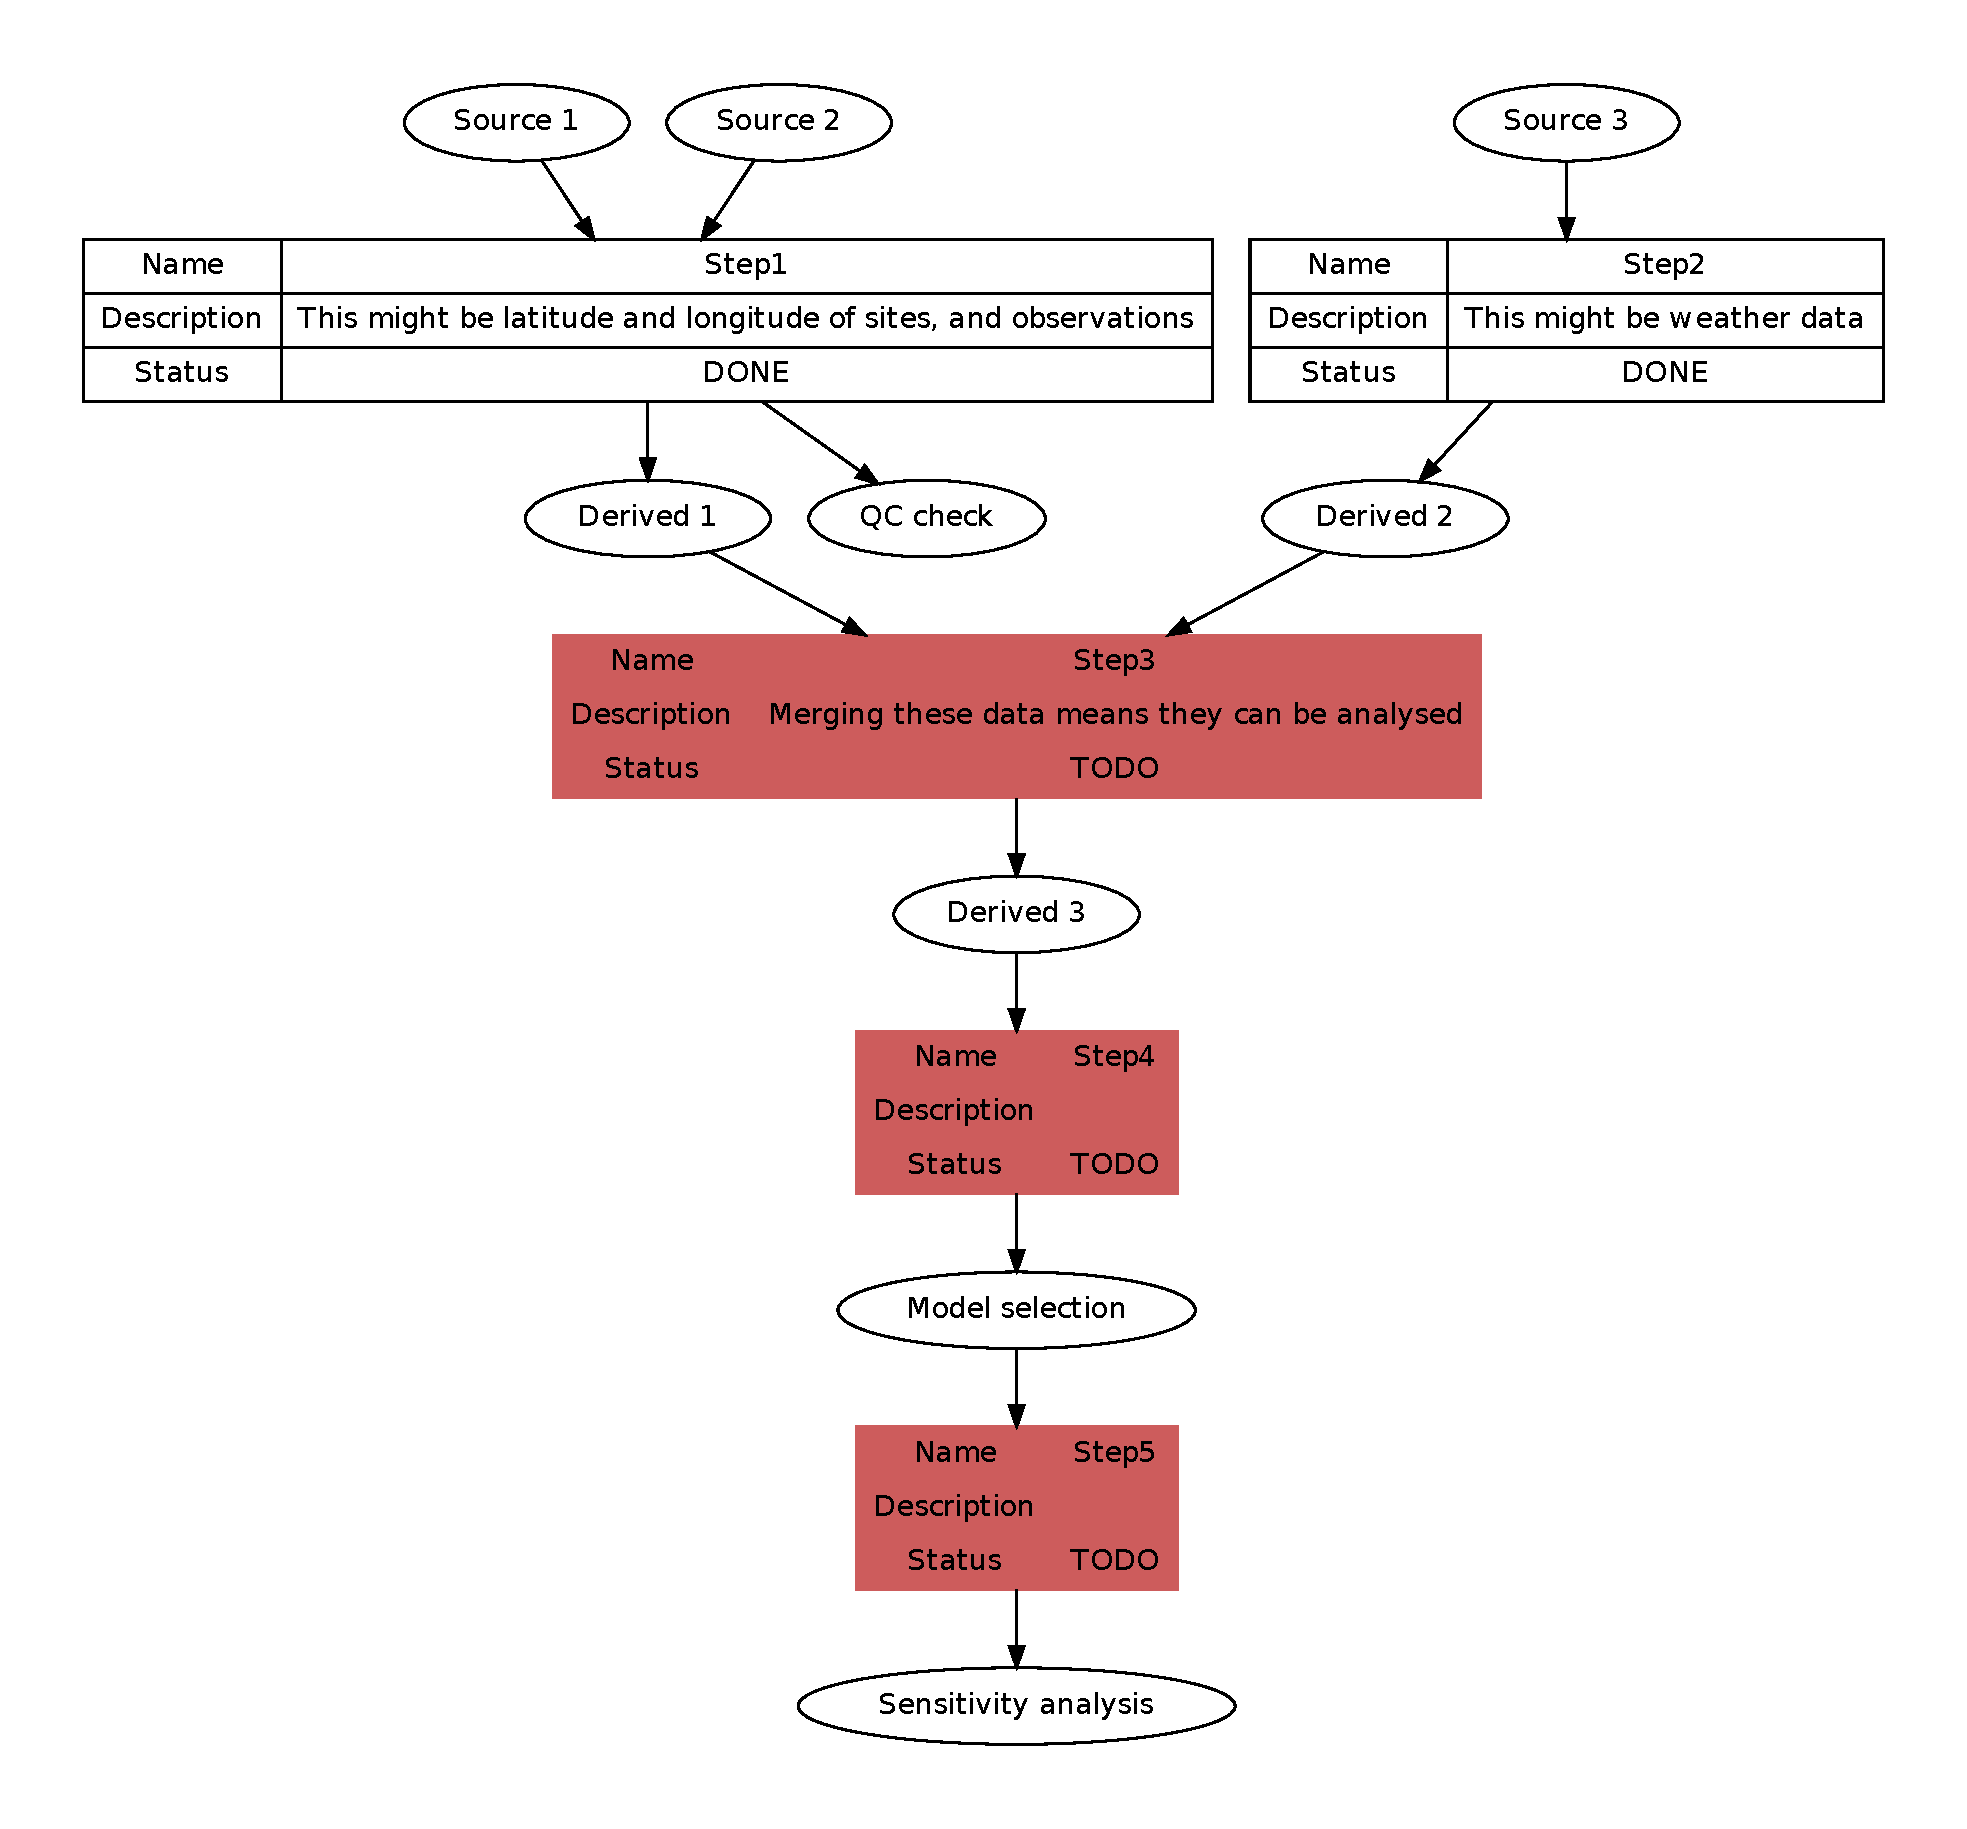
\includegraphics[width=\textwidth]{images/steps-fig1.pdf}
\caption{A visualisation of a data analysis pipeline showing the use of colour}
\label{fig:FigSteps}
\end{figure}

\clearpage

As an example of the kinds of tangible steps such a workflow might
entail a schematic diagram has been created and is shown in Figure
\ref{fig:envepi_data_pipeline.png}.

\begin{figure}[!h]
\centering
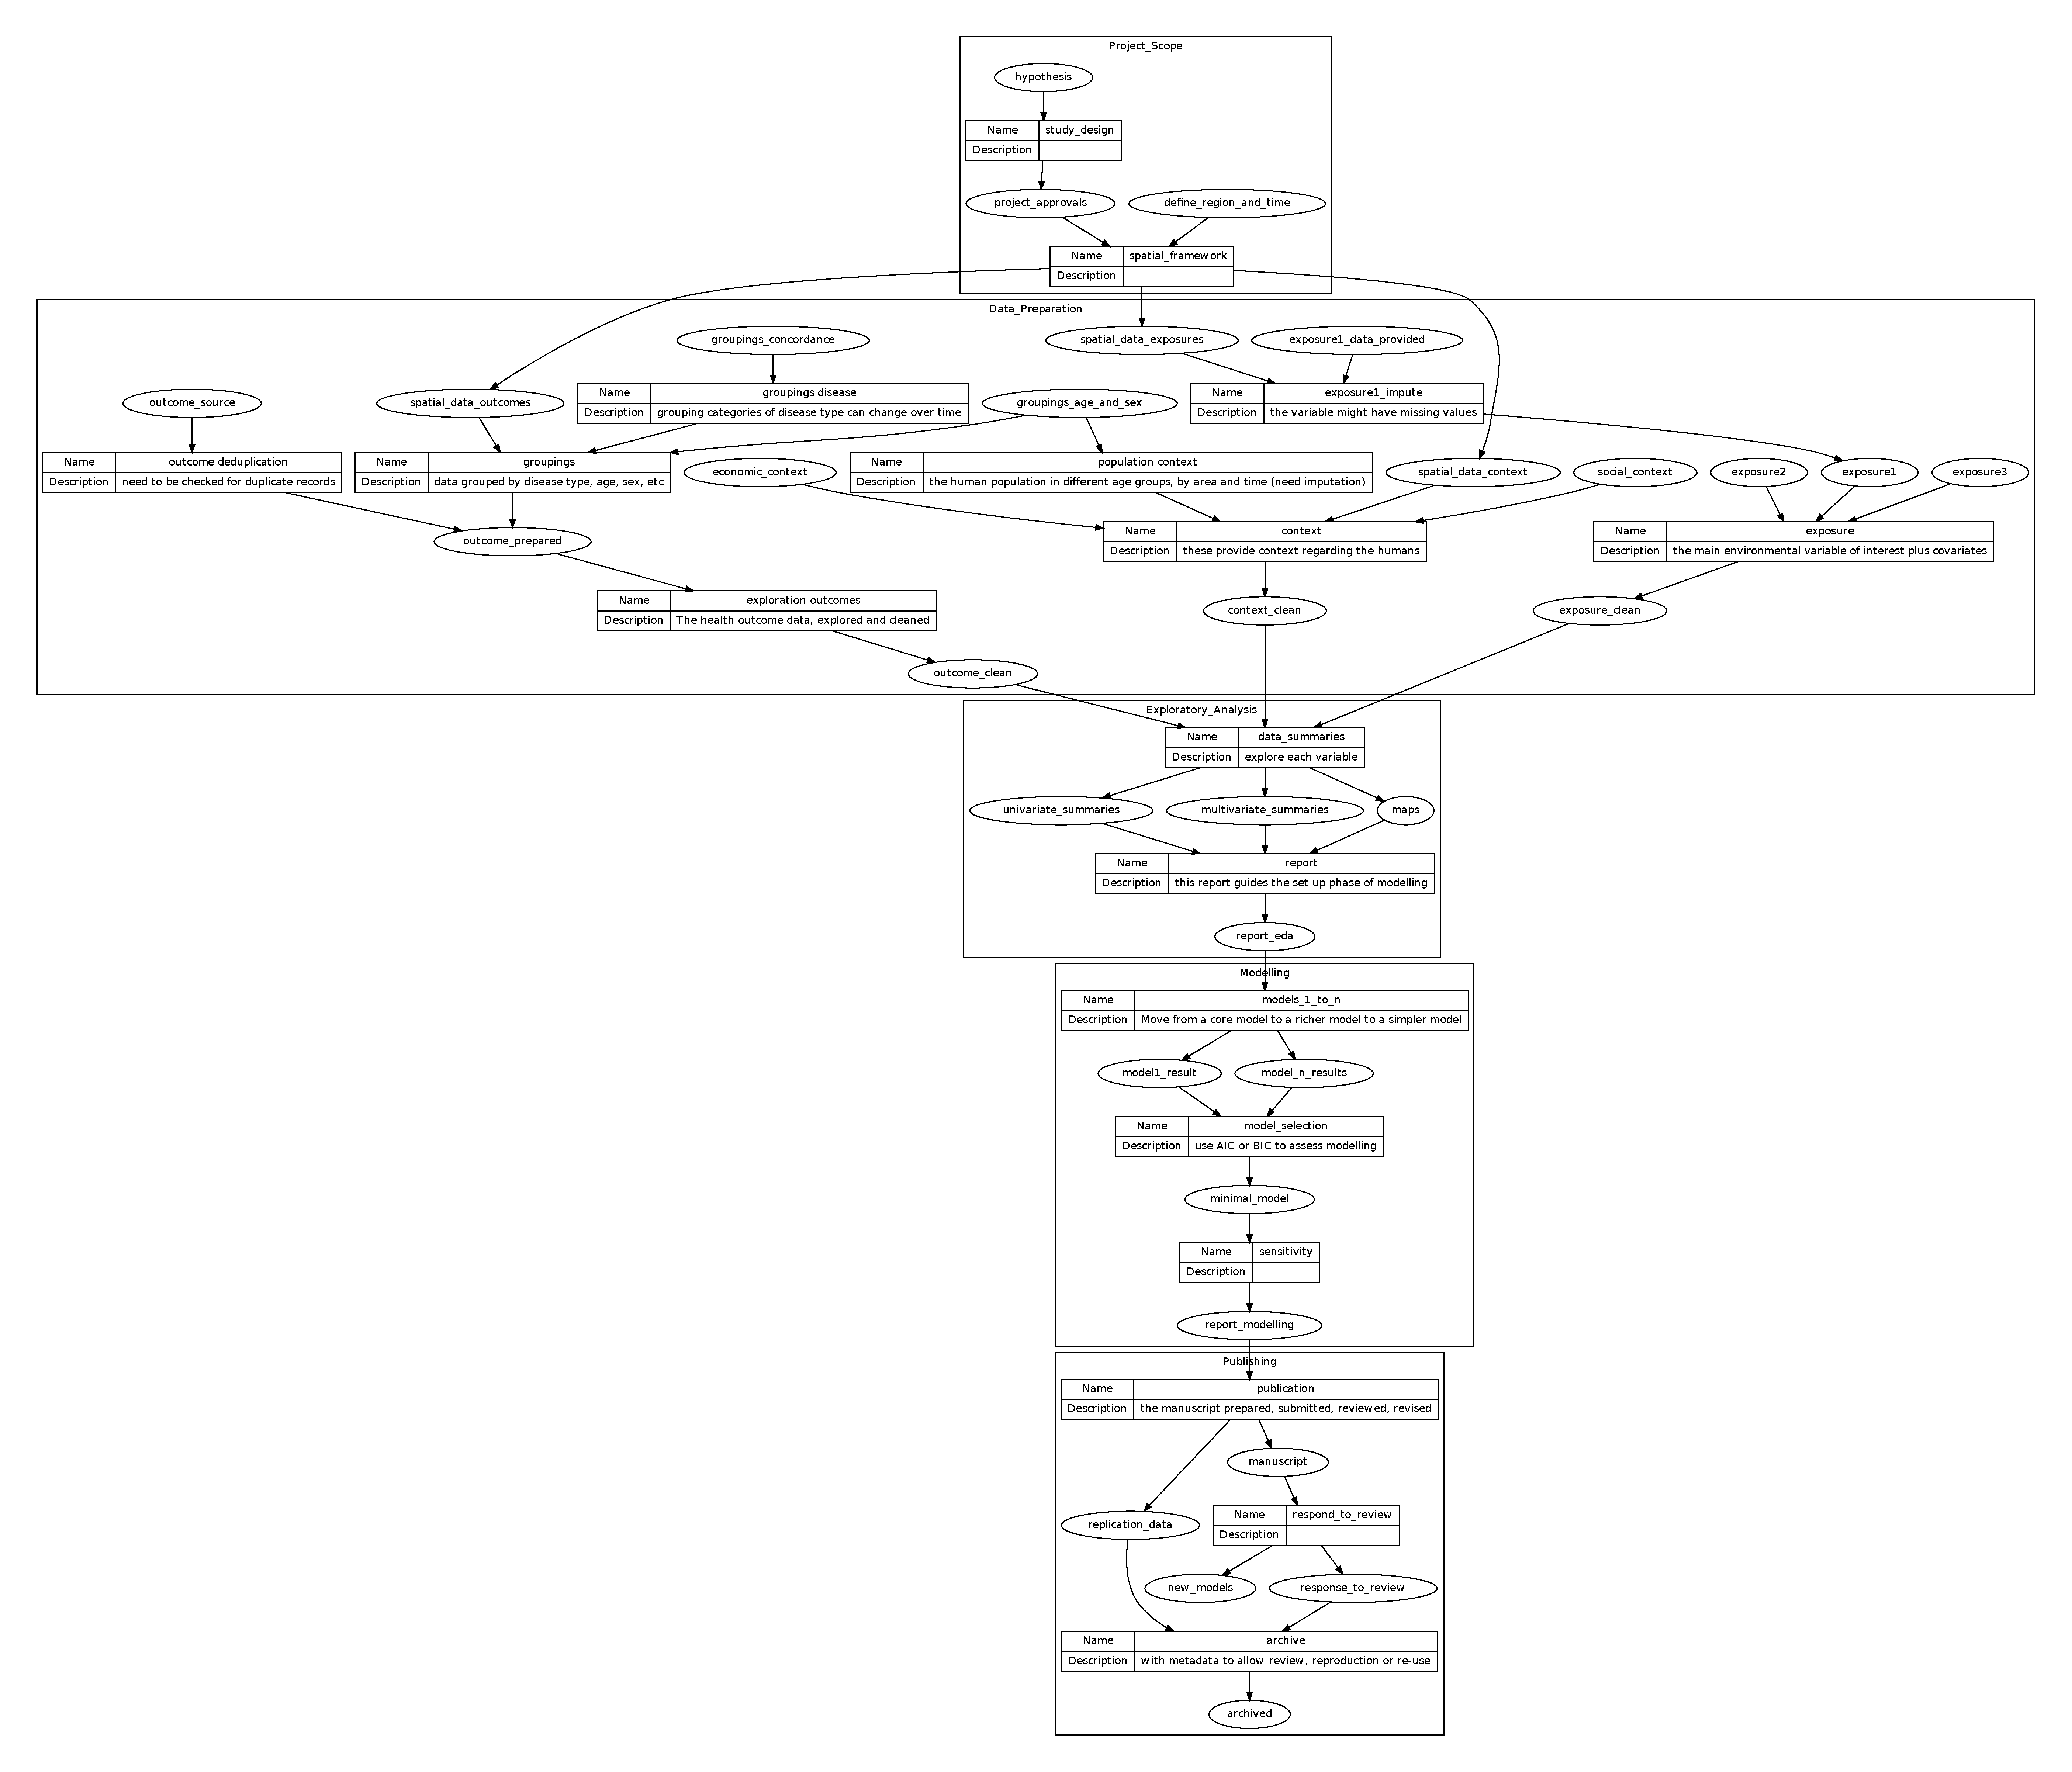
\includegraphics[width=\textwidth]{images/envepi_data_pipeline.pdf}
\caption{A schematic flow chart showing the steps required to prepare and
conduct an analysis of health, environmental and social data.}       
\label{fig:envepi_data_pipeline.png}
\end{figure}

A high resolution version of this image is available online at
\href{https://github.com/swish-climate-impact-assessment/swish_data_management_procedures/blob/phd_appendix/images/envepi_data_pipeline.pdf}{\url{https://github.com/swish-climate-impact-assessment/swish_data_management_procedures/blob/phd_appendix/images/envepi_data_pipeline.pdf}}

\subsection{Case study 3: Visualisation of methods steps using bespoke
software}\label{case-study-3-visualisation-of-methods-steps-using-bespoke-software}

The method step is the key atomic unit of a scientific pipeline. It
consists of inputs, outputs and a rationale for why the step is taken.

A simple way to keep track of the steps, inputs and outputs is shown in
Table \ref{tab:TableBasic}.

\begin{table}[!h]
\centering
\caption{A simple table to track method steps, data inputs and outputs} 
\label{tab:TableBasic}
\begin{tabular}{p{.6in}p{2in}p{2in}}
  \hline
STEP & INPUTS & OUTPUTS \\ 
  \hline
Step1 & Input 1, Input 2 & Output 1 \\ 
  Step2 & Input 3 & Output 2 \\ 
  Step3 & Output 1, Output 2 & Output 3 \\ 
   \hline
\end{tabular}
\end{table}

The steps and data listed in Table \ref{tab:TableBasic} can be
visualised. To achieve this an R function was written as part of this
PhD project and is distributed in the author's own R package available
on Github (\url{https://github.com/ivanhanigan/disentangle}). This is
the \texttt{newnode} function. The function returns a string of text
written in the \texttt{dot} language which can be rendered in R using
the \texttt{DiagrammeR} package, or the standalone \texttt{graphviz}
package. This creates the graph view shown in Figure \ref{fig:FigBasic}.
Note that a new field was added for Descriptions as these are highly
recommended.

\begin{Shaded}
\begin{Highlighting}[]
\KeywordTok{library}\NormalTok{(disentangle); }\KeywordTok{library}\NormalTok{(stringr); }\KeywordTok{library}\NormalTok{(readxl)}
\NormalTok{steps <-}\StringTok{ }\KeywordTok{read_excel}\NormalTok{(}\StringTok{"steps_basic_workflow.xlsx"}\NormalTok{)}
\NormalTok{nodes <-}\StringTok{ }\KeywordTok{newnode}\NormalTok{(}\DataTypeTok{indat =} \NormalTok{steps, }\DataTypeTok{names_col =} \StringTok{"STEP"}\NormalTok{,}
                 \DataTypeTok{in_col =} \StringTok{"INPUTS"}\NormalTok{,}\DataTypeTok{out_col =} \StringTok{"OUTPUTS"}\NormalTok{)}
\NormalTok{DiagrammeR::}\KeywordTok{grViz}\NormalTok{(nodes)}
\end{Highlighting}
\end{Shaded}

\begin{figure}[!ht]
\centering
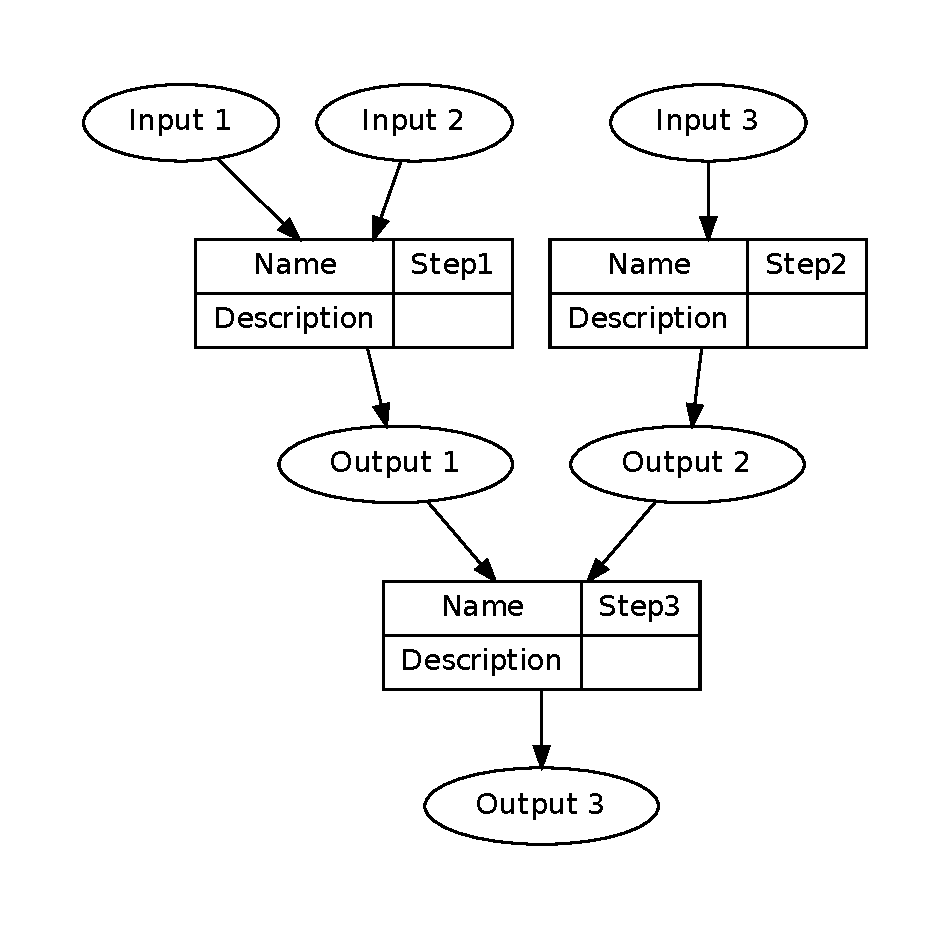
\includegraphics[width=.5\textwidth]{images/fig-basic.pdf}
\caption{A graphical view of the steps that comprise a simple data analysis pipeline}
\label{fig:FigBasic}
\end{figure}

\clearpage

\section{References for appendix 2}\label{references-for-appendix-2}

Barnett, A.G. \& Dobson, A.J. (2010). \emph{Analysing Seasonal Health
Data}. Springer, Berlin, Heidelberg, Germany.

Barnett, A.G., Baker, P. \& Dobson, A.J. (2014). Package `season':
Analysing seasonal data R functions. R package version 0.3-5.

Bodnar, A., Castorina, R., Desai, M., Duramad, P., Fischer, S., Klepeis,
N., Liang, S., Mehta, S., Naumoff, K., Noth, E.M., Schei, M., Tian, L.,
Vork, K.L. \& Smith, K.R. (2004). Lessons learned from `the skeptical
environmentalist': an environmental health perspective.
\emph{International Journal of Hygiene and Environmental Health},
207(1), 57--67.

Borer, E.T., Seabloom, E.W., Jones, M.B. \& Schildhauer, M. (2009). Some
simple guidelines for effective data management. \emph{Bulletin of the
Ecological Society of America}, (April), 205--214.

Cai, W., Cowan, T., Braganza, K., Jones, D. \& Risbey, J. (2010).
Comment on 'On the recent warming in the Murray Darling Basin: Land
surface interactions misunderstood' by Lockart et al. \emph{Geophysical
Research Letters}, 37(10), 1--3.

Fleming, L., Haines, A., Golding, B., Kessel, A., Cichowska, A., Sabel,
C., Depledge, M., Sarran, C., Osborne, N., Whitmore, C., Cocksedge, N.
\& Bloomfield, D. (2014). Data mashups: Potential contribution to
decision support on climate change and health. \emph{International
Journal of Environmental Research and Public Health}, 11(2), 1725--1746.

Leek, J.T. \& Peng, R.D. (2015). Statistics: P values are just the tip
of the iceberg. \emph{Nature}, 520(7549), 612--612.

McMichael, A.J. (2013). Impediments to comprehensive research on climate
change and health. \emph{International Journal of Environmental Research
and Public Health}, 10(11), 6096--6105.

Michener, W.K., Brunt, J.W., Helly, J.J., Kirchner, T.B. \& Stafford,
S.G. (1997). Nongeospatial metadata for the ecological sciences.
\emph{Ecological Applications}, 7(1), 330--342.

Noble, W.S. (2009). A quick guide to organizing computational biology
projects. \emph{PLoS Computational Biology}, 5(7), 1--5.

O'Keefe, B. (2007). Hackers pick up UQ cash prize. \emph{The
Australian}.
\url{http://www.theaustralian.com.au/higher-education/hackers-pick-up-uq-cash-prize/story-e6frgcjx-1111113191659}
{[}Accessed 14 Oct. 2015{]}

Peng, R.D. (2015). \emph{Report Writing for Data Science in R}. Leanpub.
Unpublished Draft (Accessed 22 Dec. 2015).
\url{https://leanpub.com/reportwriting}

Peng, R.D. \& Dominici, F. (2008). \emph{Statistical Methods for
Environmental Epidemiology with R. A Case Study in Air Pollution and
Health}. Springer Science \& Business Media, New York, USA.

Peng, R.D., Dominici, F. \& Zeger, S.L. (2006). Reproducible
epidemiologic research. \emph{American Journal of Epidemiology}, 163(9),
783--789.

Pullin, A.S. \& Salafsky, N. (2010). Save the whales? Save the
rainforest? Save the data! \emph{Conservation Biology}, 24(4), 915--917.

Schwab, M., Karrenbach, M. \& Claerbout, J. (2000). Making scientific
computations reproducible. \emph{Computing in Science and Engineering},
2(6), 61--67.

Silberzahn, R. \& Uhlmann, E.L. (2015). Crowdsourced research: Many
hands make tight work. \emph{Nature}, 526(7572), 189--191.

Vines, T.H., Albert, A.Y.K., Andrew, R.L., D{\a'e}barre, F., Bock, D.G.,
Franklin, M.T., Gilbert, K.J., Moore, J.-S., Renaut, S. \& Rennison,
D.J. (2014). The availability of research data declines rapidly with
article age. \emph{Current Biology}, 24(1), 94--97.

White, E., Baldridge, E., Brym, Z., Locey, K., McGlinn, D. \& Supp, S.
(2013). Nine simple ways to make it easier to (re)use your data.
\emph{Ideas in Ecology and Evolution}, 6(2), 1--10.

Wickham, H. (2014). Tidy data. \emph{Journal of Statistical Software},
59(10), 1--23.

Xie, Y. (2014). Chapter 1. Knitr: A comprehensive tool for reproducible
research in R. \emph{Implementing Reproducible Research} (eds V.
Stodden, F. Leisch \& R. Peng). CRC Press, Boca Raton, USA.

\end{document}